\documentclass{standalone}
\usepackage{tikz}
\usetikzlibrary{calc,patterns,decorations.pathmorphing,decorations.markings}
\usepackage{graphicx}

\begin{document}

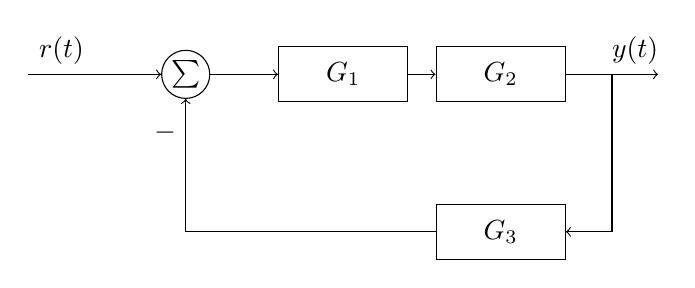
\begin{tikzpicture}[node distance=20mm, block/.style={rectangle, draw, text width=1.5cm, align=center, minimum height = 0.7cm, inner sep=2pt},]
   \node[coordinate] (input) {};
   \node[circle, draw, right of=input, inner sep=1pt] (sum) {$\sum$};
   \node[block, right of=sum, ] (G1) {$G_1$};
   \node[block, right of=G1] (G2) {$G_2$};
   \node[block, below of=G2] (G3) {$G_3$};
   \node[coordinate, right of=G2] (output) {};
   \draw[->] (input) -- node[near start, above] {$r(t)$}  (sum);
   \draw[->] (G2) -- node[coordinate] (measure) {} node[near end, above] {$y(t)$} (output);
   \draw[->] (sum) --  (G1);
   \draw[->] (G1) --  (G2);
   \draw[->] (measure) |-  (G3);
   \draw[->] (G3) -| node [very near end, left] {$-$}  (sum);
   
 \end{tikzpicture}
 
\end{document}
 